%"The PDF file may contain up to 25 pages of reference material, single-sided, letter or A4 size, with text and illustrations readable by a person with correctable eyesight without magnification from a distance of 1/2 meter."
\documentclass[10pt,landscape,twocolumn,a4paper,notitlepage]{article}
\usepackage{hyperref}
\usepackage[english, activeacute]{babel}
\usepackage[utf8]{inputenc}
\usepackage{fancyhdr}
\usepackage{lastpage}
\usepackage{listings}
\usepackage{amssymb}
\usepackage[usenames,dvipsnames]{color}
\usepackage{graphicx}
\usepackage{wrapfig}
\usepackage{amsmath}
\usepackage{makeidx}

%%% Margenes
\setlength{\columnsep}{0.25in}    % default=10pt
\setlength{\columnseprule}{0.5pt}    % default=0pt (no line)

\addtolength{\textheight}{2.35in}
\addtolength{\topmargin}{-0.9in}     % ~ -0.5 del incremento anterior

\addtolength{\textwidth}{1.1in}
\addtolength{\oddsidemargin}{-0.55in} % -0.5 del incremento anterior

\setlength{\headsep}{0.08in}
\setlength{\parskip}{0in}
\setlength{\headheight}{15pt}
\setlength{\parindent}{0mm}

%%% Encabezado y pie de pagina
\pagestyle{fancy}
\fancyhead[LO]{\textbf{\title}}
\fancyhead[C]{\leftmark\ -\ \rightmark}
\fancyhead[RO]{Page \thepage\ of \pageref{LastPage}}
\renewcommand{\headrulewidth}{0.4pt}
\fancyfoot{}
\definecolor{darkblue}{rgb}{0,0,0.4}
%%% Configuracion de Listings
\lstloadlanguages{C++}
\lstnewenvironment{code}
	{%\lstset{	numbers=none, frame=lines, basicstyle=\small\ttfamily, }%
	 \csname lst@SetFirstLabel\endcsname}
	{\csname lst@SaveFirstLabel\endcsname}
\lstset{% general command to set parameter(s)
	language=C++, basicstyle=\small\ttfamily, keywordstyle=\slshape,
	emph=[1]{tipo,usa}, emphstyle={[1]\sffamily\bfseries},
	morekeywords={tint,forn,forsn,fore},
	basewidth={0.47em,0.40em},
	columns=fixed, fontadjust, resetmargins, xrightmargin=5pt, xleftmargin=15pt,
	flexiblecolumns=false, tabsize=2, breaklines,	breakatwhitespace=false, extendedchars=true,
	numbers=left, numberstyle=\tiny, stepnumber=1, numbersep=9pt,
	frame=l, framesep=3pt,
    basicstyle=\ttfamily,
    keywordstyle=\color{darkblue}\ttfamily,
    stringstyle=\color{magenta}\ttfamily,
    commentstyle=\color{RedOrange}\ttfamily,
    morecomment=[l][\color{OliveGreen}]{\#}
}

\lstdefinestyle{C++}{
	language=C++, basicstyle=\small\ttfamily, keywordstyle=\slshape,
	emph=[1]{tipo,usa,tipo2}, emphstyle={[1]\sffamily\bfseries},
	morekeywords={tint,forn,forsn,fore},
	basewidth={0.47em,0.40em},
	columns=fixed, fontadjust, resetmargins, xrightmargin=5pt, xleftmargin=15pt,
	flexiblecolumns=false, tabsize=2, breaklines,	breakatwhitespace=false, extendedchars=true,
	numbers=left, numberstyle=\tiny, stepnumber=1, numbersep=9pt,
	frame=l, framesep=3pt,
    basicstyle=\ttfamily,
    keywordstyle=\color{darkblue}\ttfamily,
    stringstyle=\color{magenta}\ttfamily,
    commentstyle=\color{RedOrange}\ttfamily,
    morecomment=[l][\color{OliveGreen}]{\#}
}

%%% Macros
\def\nbtitle#1{\begin{Large}\begin{center}\textbf{#1}\end{center}\end{Large}}
\def\nbsection#1{\section{#1}}
\def\nbsubsection#1{\subsection{#1}}
\def\nbcoment#1{\begin{small}\textbf{#1}\end{small}}
\newcommand{\comb}[2]{\left( \begin{array}{c} #1 \\ #2 \end{array}\right)}
\def\complexity#1{\texorpdfstring{$\mathcal{O}(#1)$}{O(#1)}}
 \newcommand\pyfile[2][]{
\lstinputlisting[language=Python,linerange={#1}]{#2}}

\begin{document}
\def\title{Notebook Python}
.\\[0.2cm]
\centering{\LARGE\textbf{Estufa en Piloto}} \\[0.5cm]
\centering{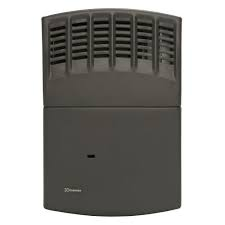
\includegraphics[width=5.5cm]{img/estufa.jpeg}}
\tableofcontents\newpage

\section{Basic}
\subsection{Binary Search}
\pyfile{Basic/binsearch.py}
\subsection{LIS}
\subsubsection{Naive}
\pyfile{Basic/LIS.py}
\subsubsection{Fast}
\pyfile{Basic/fastLIS.py}
\newpage
\section{Data Structures}

\subsection{DSU}
\pyfile{"Data Structures/dsu.py"}
\subsection{FenwickTree}
\pyfile{"Data Structures/FenwickTree.py"}
\subsection{Segment Tree}
\pyfile{"Data Structures/segmenttree.py"}
\subsection{Sparse Table}
\pyfile{"Data Structures/sparsetable.py"}
\newpage
\section{Graph}
\subsection{BFS}
\pyfile{Graph/bfs.py}
\subsection{DFS}
\pyfile{Graph/dfs.py}
\subsection{Dijkstra}
\pyfile{Graph/Dijkstra.py}
\subsection{Floyd-Warshall}
\pyfile{Graph/floydwarshall.py}
\subsection{Max Flow-Min Cut (Ford Fulkerson)}
\pyfile{Graph/flow.py}




\newpage
\section{Math}
\subsection{Identities}
{
$C_n = \frac{2(2n-1)}{n+1} C_{n-1}$

$C_n = \frac{1}{n+1} \binom{2n}{n}$

$C_n \sim \frac{4^n}{n^{3/2}\sqrt{\pi}}$

$\sigma(n) = O(\log(\log(n)))$ (number of divisors of $n$)

$F_{2n+1} = F_{n}^2 + F_{n+1}^2$

$F_{2n} = F_{n+1}^2 - F_{n-1}^2$

$\sum_{i=1}^n F_i = F_{n+2}-1$

$F_{n+i}F_{n+j} - F_nF_{n+i+j} = (-1)^n F_iF_j$

$\sum_{i=1}^{n} i^k = \frac{1}{k+1}(\sum_{j=1}^{k+1}\binom{k+1}{j}n^j-\sum_{j=0}^{k-1}\binom{k+1}{j}i^j)$
$S_k(n)= \frac{1}{k+1}((n+1)^{k+1}-1-(\sum_{j=2}^{k+1}\binom{k+1}{j}S_{k+1-j}(n)))$

(Möbius Inv. Formula)
Let $g(n) = \sum_{d\mid n} f(d)$, then $f(n)=\sum_{d\mid n} g(d) \mu\left(\frac{n}{d}\right)$.
}
\subsection{GCD}
\pyfile{Math/gcd.py}
\subsection{Euler Totient (Phi)}
\pyfile{Math/totient.py}
\subsection{Extended Euclides}
\pyfile{Math/ext_euclides.py}
\subsection{Modexp}
\pyfile{Math/modexp.py}
\subsection{allModInv}
\pyfile{Math/allModInv.py}
\subsection{Iter multiplication}
\pyfile{Math/itermul.py}

\subsection{Test de primalidad y Descomposicion en Primos}
\subsubsection{Is Prime}
\pyfile{Math/is_prime.py}
\subsubsection{Miller Rabin Test}
\pyfile{Math/millerRabinTest.py}
\subsubsection{Prime Factors}
\pyfile{Math/primefactors.py}
\subsubsection{Integer Fact}
\pyfile{Math/integer_fact.py}


\subsection{Diofanticas}
\pyfile{Math/diophantine.py}

\subsection{Cribas}
\subsubsection{Criba Primos}
\pyfile{Math/criba_primos.py}
\subsubsection{Block Sieving}
\pyfile{Math/block_sieving.py}
\subsubsection{Linear Sieve}
\pyfile{Math/linear_sieve.py}

\subsection{Divisores}
\subsubsection{Count Divisors}
\pyfile{Math/count_div.py}
\subsubsection{Suma Divisores}
\pyfile{Math/divisors_sum.py}

\subsection{Factorial}
\subsubsection{Factorial mod}
\pyfile{Math/factmod.py}
\subsubsection{Factorial Divisors}
\pyfile{Math/factorial_divisors.py}

\subsection{FFT}
\pyfile{Math/FFT.py}
\subsection{Lagrange Interpolation}
\pyfile{Math/lagrange.py}


\subsection{Discrete Log}
\pyfile{Math/discretelog.py}
\subsection{Discrete Root}
\pyfile{Math/discreteroot.py}
\subsection{Primitive Root}
\pyfile{Math/primitiveroot.py}
\subsection{Fibonacci}
\pyfile{Math/fibo.py}
\subsection{Gray Code}
\pyfile{Math/graycode.py}

\subsection{Matrix}
\pyfile{Math/matrix/matrix_sum.py}
\pyfile{Math/matrix/matrix_sum.py}

\newpage
\section{Geo}
\subsection{Convex Hull}
\pyfile{Math/geo/convexhull.py}
\subsection{Determinant}
\pyfile{Math/geo/determinant.py}
\subsection{GreatCircleDistance}
\pyfile{Math/geo/greatCircleDistance.py}
\subsection{Perimeter}
\pyfile{Math/geo/perimeter.py}
\subsection{Turn}
\pyfile{Math/geo/turn.py}

\newpage
\section{Strings}
\subsection{Hash}
\pyfile{Strings/hash.py}
\subsection{Prefix Function}
\pyfile{Strings/prefixFunction.py}
\subsection{KMP}
\pyfile{Strings/KMP.py}
\subsection{Rabin Karp}
\pyfile{Strings/rabinkarp.py}
\subsection{Aplicaciones de KMP y Rabin}
\pyfile{Strings/applications.py}
\subsection{Unique Substrings}
\pyfile{Strings/countUniqueSubstrings.py}
\subsection{Group Identical Strings}
\pyfile{Strings/groupIdenticalStrings.py}
\newpage
\section{Tricks With Bits}
\begin{verbatim}
In python3, ~x (flip all bits in other languages) is achieved with
(~x & 0xFFFFFFFF) (use repit1 lenght of HEXA as you wish)


x & (x-1)
clear the lowest set bit of x
x & ~(x-1)
extracts the lowest set bit of x (all others are clear).
Pretty patterns when applied to a linear sequence.
x & (x + (1 << n))
the run of set bits (possibly length 0) starting at bit n cleared.
x & ~(x + (1 << n))
the run of set bits (possibly length 0) in x, starting at bit n.
x | (x + 1)
x with the lowest cleared bit set.
x | ~(x + 1)
Extracts the lowest cleared bit of x (all others are set),
if ~ wrapping the expression, you have that cleared value.
x | (x - (1 << n))
x With the run of cleared bits (possibly length 0) starting at bit n set.
x | ~(x - (1 << n))
The lowest run of cleared bits (possibly length 0) in x,
starting at bit n are the only clear bits.


By 'run' is intended the number formed by all consecutive
1's at the left of n-th bit, starting at n-th bit.
\end{verbatim}

\newpage



\section{Plantilla}
\pyfile{plantilla.py}































\end{document}
